\documentclass[11pt,aspectratio=43,ignorenonframetext,t]{beamer}
% Uses fontspec - assumes compiled with LuaLaTeX or similar
% The above \documentclass is for making slides. If making handouts use:
%\documentclass[11pt,a4paper]{article} 
%\usepackage{beamerarticle}
%\setjobnamebeamerversion{main.beamer}

% See https://github.com/CASSON-LAB/uom_beamer_template
% for details on license, further useage information and similar
%%%%%%%%%%%%%%%%%% DOCUMENT SETUP %%%%%%%%%%%%%%%%%%

% Presentation settings
\mode<presentation>{
  \usetheme[framenumber,titleframestart=1]{UoM_alex}
  \usefonttheme{professionalfonts} % using non standard fonts for beamer
  \usefonttheme{serif}             % set font to Arial
  \usepackage{fontspec}
  \setmainfont[Ligatures=TeX]{Arial}
}

% Handout settings
\mode<article>{
  \usepackage{fullpage}                  % use full page
  \usepackage{fontspec}                  % set font to Arial
    \setmainfont[Ligatures=TeX]{Arial}
  \setlength{\parskip}{1.5\baselineskip} % correct beamer line spacings
  \setlength{\parindent}{0cm}
  \usepackage{enumitem}
    \setlist[itemize]{topsep=0pt}
  \definecolor{uomlinkblue}{HTML}{0071BC}
}


% Packages

% Configurando layout para mostrar codigos C++
\usepackage{listings}
\lstset{
  language=HTML,
  basicstyle=\ttfamily\small, 
  keywordstyle=\color{blue}, 
  stringstyle=\color{red}, 
  commentstyle=\color{red}, 
  extendedchars=true, 
  showspaces=false, 
  showstringspaces=false, 
  numbers=left,
  numberstyle=\tiny,
  breaklines=true, 
  backgroundcolor=\color{green!10},
  breakautoindent=true, 
  captionpos=b,
  xleftmargin=0pt,
}

\usepackage{graphicx}  % for graphics files
  \graphicspath{./fig/aula9}
\usepackage{amsmath}   % assumes amsmath package installed
  \allowdisplaybreaks[1] % allow eqnarrays to break across pages
\usepackage{amssymb}   % assumes amsmath package installed 
\usepackage{hyperref} % add hyperlinks to document. Settings are for accessiblity
  \hypersetup{
    colorlinks=true,
    linkcolor=uomlinkblue,
    filecolor=uomlinkblue,      
    urlcolor=uomlinkblue,
	pdflang={en-GB},
}
\usepackage[document]{ragged2e} % left aligned text for accessibility
% experimental - does fundamentally work, if with quite a bit of effort
%\usepackage{axessibility} % LaTeX readable equations for accessibility
%  \tagpdfsetup{tabsorder=structure,uncompress,activate-all,interwordspace=true}
%  \pdfextension catalog{/Lang (en-GB)}
%  \RequirePackage{luacode}
%  \directlua{require("axessibility.lua")}
\usepackage{unicode-math} % unicode maths for accessibility
\usepackage{pdfcomment} % for alt text for accessibility
\usepackage{rotating}  % allow portrait figures and tables
\usepackage{subfigure} % allow matrices of figures
\usepackage{float}     % allows H option on floats to force here placement
\usepackage{multirow}  % allows merging of rows in tables
\usepackage{tabularx}  % allows fixed width tables
\usepackage{ctable}    % modifies \hline for use in table
\usepackage{bm}        % allow bold fonts in equations
\usepackage{pgf}       % allow graphics manipulation
\usepackage{media9}    % allow interactive flash files to be embedded
  \addmediapath{../media}
\usepackage{etoolbox}
  \makeatletter \preto{\@verbatim}{\topsep=0pt \partopsep=0pt} \makeatother  
  
% Custom commands
\newcommand{\matlab}{\emph{\sc{Matlab}}}
\newcommand{\maple}{\emph{\sc{Maple}}}
\newcommand{\simulink}{\emph{\sc{Simulink}}}
\newcommand{\dc}{d.c.}
\newcommand{\ac}{a.c.}
\newcommand{\rms}{RMS}
\newcommand{\wgn}{{\tt wgn}}
\newcommand{\sus}[1]{$^{\mbox{\scriptsize #1}}$}
\newcommand{\sub}[1]{$_{\mbox{\scriptsize #1}}$}
\newcommand{\chap}[1]{Chapter~\ref{#1}}
\newcommand{\sect}[1]{Section~\ref{#1}}
\newcommand{\fig}[1]{Fig.~\ref{#1}}
\newcommand{\tab}[1]{Table~\ref{#1}}
\newcommand{\equ}[1]{(\ref{#1})}
\newcommand{\appx}[1]{Appendix~\ref{#1}}
\newcommand{\degree}{\ensuremath{^\circ}}
\newcommand{\Vrms}{Vrms}
\newcommand{\Vpp}{V\sub{pp}}
\newcommand{\otoprule}{\midrule[\heavyrulewidth]}         
\newcolumntype{Z}{>{\centering\arraybackslash}X}  % tabularx centered columns 
\makeatletter \DeclareRobustCommand{\em}{\@nomath\em \if b\expandafter\@car\f@series\@nil \normalfont \else \bfseries \fi} \makeatother
\newcounter{example_number} % keep track of the example questions



%%%%%%%%%%%%%%%%%% FRONT MATTER %%%%%%%%%%%%%%%%%%
\title{Desenvolvimento de Software}
\subtitle{Aula 7}
\author{Prof. Me. Juliana Costa-Silva}

\begin{document}

\maketitle
%%%%%%%%%%%%%%%%%% TITLE SLIDE %%%%%%%%%%%%%%%%%%
\mode<presentation>{ \frame{\titlepage \label{slide:a}}} 
%\begin{figure}[!ht] 
%\fbox{\includeslide[width=\textwidth]{slide:a}} \end{figure}

%------------------------------------------------------------------------
\mode<presentation>{
\begin{frame}
\frametitle{Na aula de hoje...} 
\tableofcontents 
\end{frame}
}

%------------------------------------------------------------
\mode<presentation>{
\section{Encapsulamento}
\begin{frame}{Encapsulamento}
  \begin{block}{Encapsulamento}
      Conceitua-se encapsulamento como sendo o processo utilizado para proteger os campos e operações de uma classe (atributos e métodos), permitindo que apenas os membros públicos - em Java métodos Get / Set - sejam acessados pelos usuários de determinada classe.
  \end{block}
\end{frame}}
%------------------------------------------------------------
\mode<presentation>{
\begin{frame}{Encapsulamento}
  \begin{block}{Encapsulamento}
  Vantagens do encapsulamento: \\
      \begin{enumerate}
          \item \textbf{Segurança} - a comunicação só é feita por métodos modificadores de acesso, desta forma pode-se prevenir que usuários não autorizados vejam ou modifiquem algum campo protegido da classe;
          \item \textbf{Manutenção} - facilita a manutenção da classe pois ela pode ser feita de forma isolada;
          \item \textbf{Reduz acoplamento} - Quanto menor o acoplamento entre classes, maior pode ser a reutilização dessa classe.
      \end{enumerate}
  \end{block}
\end{frame}}
%------------------------------------------------------------
\mode<presentation>{
\section{Operadores de Visibilidade}
\begin{frame}{Operadores de visibilidade}
\begin{block}{Público - public}
    Nível de acesso livre. Indica que o método ou atributo da classe é público, ou seja, pode-se acessar este atributo, ou executar esse método, por qualquer código de programa. Usamos o sinal (+) na notação UML para simbolizar essa visibilidade.
\end{block}
\begin{block}{Privado - private}
    Nível mais protegido. Membros declarados como private, só podem ser acessados dentro da classe em que foram declarados. Usamos o sinal (-) na notação UML para simbolizar essa visibilidade.
\end{block}
\end{frame}}
%------------------------------------------------------------
\mode<presentation>{
\begin{frame}{Operadores de visibilidade [2]}
\begin{block}{Protegido - protected}
    Nível de acesso intermediário. Serve para que o método ou o atributo seja público dentro do código da própria classe e de qualquer classe que herde daquela onde está o método ou propriedade protected. É privado e não acessível de qualquer outra parte. Usamos o sinal (\#) na notação UML para simbolizar essa visibilidade.
\end{block}
\end{frame}}
%--------------------------------------------------------
\mode<presentation>{
\section{Get e Set}
\begin{frame}{Manipulando atributos}

        E se precisarmos alterar apenas o valor de um atributo \textbf{privado}?\\

  Para manipular valores de atributos, a classe deve possuir métodos get e set para cada um de seus atributos.\\
\pause
\textcolor{red}{Podemos receber valores sem validar?}\\ Vamos desenvolver os métodos get e set da classe Conta, como atividade extra, faça a validação.
  

\end{frame}}
%--------------------------------------------------------
\mode<presentation>{
\begin{frame}{Manipulando atributos}

        \begin{center}
        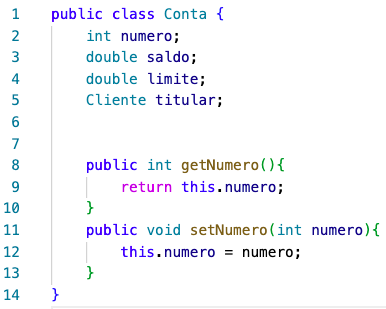
\includegraphics[height=0.8\paperheight]{fig/aula7/getSet_aula7.png} \\
        \end{center}
  

\end{frame}}

%--------------------------------------------------------
\mode<presentation>{
\begin{frame}{Voltando ao banco...}
  Também é possível associar um valor padrão (\textit{default}) para nossos atributos.\\
\begin{center}
  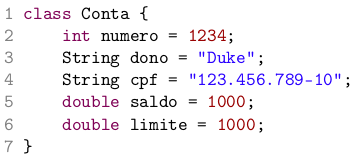
\includegraphics[height=0.3\paperheight]{fig/aula9/conta2.png} \\
 \end{center}
Nesse caso os atributos de um objeto são populados com os valores definidos na declaração dos atributos, e ao criarmos um objeto ele já esta populado.
\end{frame}}
%----------------------------------------------------------------------------
\mode<presentation>{
\begin{frame}{Cliente.java e Conta.java}
  Um atributo também pode ser uma referência para outra classe.\\
  Vejamos a classe cliente:
  \begin{columns}
    \begin{column}{0.4\textwidth}
      \begin{center}
	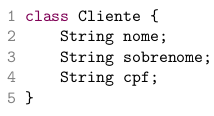
\includegraphics[height=0.25\paperheight]{fig/aula9/cliente.png} \\
      \end{center}
   \end{column}
   \begin{column}{0.4\textwidth}
      \begin{center}
	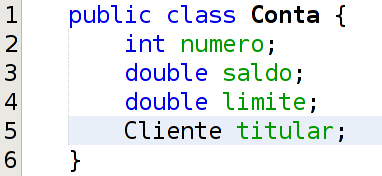
\includegraphics[height=0.2\paperheight]{fig/aula9/contaCliente.png} \\
      \end{center}
   \end{column}

  \end{columns}
Objetos que possuem referência a outras classes, são chamados de objetos compostos.
\end{frame}}
%----------------------------------------------------------------------------
\mode<presentation>{
\begin{frame}{Teste.java}
  \begin{center}
      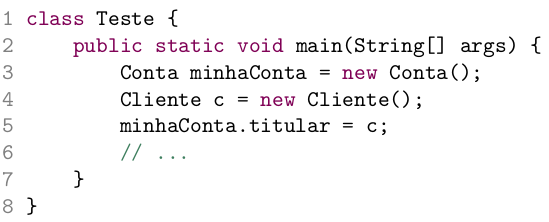
\includegraphics[height=0.35\paperheight]{fig/aula9/contaClienteMain.png} \\
  \end{center}
  \pause
  Aqui, simplesmente houve uma atribuição. \\ 
  O valor da variável c é copiado para  o atributo titular do objeto ao qual minhaConta se refere. \\ 
Em outras palavras, minhaConta agora tem uma referência ao mesmo Cliente que c se refere, e pode ser acessado através de minhaConta.titular.  
\end{frame}}
%----------------------------------------------------------------------------
\mode<presentation>{
\begin{frame}{Funcionario.java}
Vejamos a classe que registra os funcionários do banco.
 \small{ 
\lstinputlisting[linerange={2-7}]{./cod/Banco/Funcionario.java}}
\pause Crie os métodos get e set para cada atributo da classe.
\end{frame}}
%----------------------------------------------------------------------------
\mode<presentation>{
\begin{frame}{Gerente.java}
Vejamos a classe que registra os Gerentes do banco.
 \small{ 
\lstinputlisting[linerange={3-20}]{./cod/Banco/noExtended/Gerente.java}}
\pause
Repetimos alguns trechos de código?
\end{frame}}
%----------------------------------------------------------------------------
\mode<presentation>{
\begin{frame}{Pensando...}
\begin{itemize}
 \item E se tivéssemos mais algum tipo de funcionário?
 \pause \item Se for necessário guardar mais alguma informação sobre todos os 
funcionários? Teríamos que editar todas as classes (Funcionario, Gerente, 
Tipo3...)
  \pause \item Existe uma maneira de relacionarmos uma classe de tal maneira que 
  uma delas \textbf{herda} tudo que a outra tem. 
  \pause \item Isto é uma relação de \underline{classe mãe} e \underline{classe 
    filha}. 
   \pause \item No nosso caso, gostaríamos de fazer com que o Gerente tivesse 
tudo que um Funcionario tem, gostaríamos que ela fosse uma extensão de  
Funcionario. 
\pause \item Fazemos isto através da palavra chave \textit{extends}.
\end{itemize}

\end{frame}}

%----------------------------------------------------------------------------
\section{Herança}
\mode<presentation>{
\begin{frame}{Herança}
 \small{ 
\lstinputlisting[linerange={1-13}]{./cod/Banco/Gerente.java}}
\end{frame}}

%----------------------------------------------------------------------
\mode<presentation>{
\begin{frame}{Utilizando a nova classe Gerente}
 \small{ 
\lstinputlisting[linerange={1-8}]{./cod/Banco/TestaGerente.java}}\pause
\vspace{0.3cm}
\begin{block}{Super e Sub classe}
 A nomenclatura mais encontrada é que Funcionario é a 
superclasse de Gerente, e Gerente é a subclasse de Funcionario. Dizemos também que todo Gerente é um Funcionário.
\end{block}

\end{frame}}

%----------------------------------------------------------------------
\section{Reescrita de métodos}
\mode<presentation>{
\begin{frame}{Funcionario.java}
Como controlar a bonificação dos funcionários?\\
\pause
Vamos criar o método bonificação:
\small{ 
\lstinputlisting[linerange={8-10}]{./cod/Banco/Funcionario.java}}
\pause
Porém queremos que Gerentes tenham uma bonificação de 15\% e os outros 
funcionários uma bonificação de 10\%.
\pause
\textbf{Teste a bonificação de Gerente e Funcionário.}
\end{frame}}
%----------------------------------------------------------------------
\mode<presentation>{
\begin{frame}{Reescrita de métodos}
 Na classe Gerente.java reescreva o método getBonificacao().
  \small{ 
\lstinputlisting[linerange={17-19}]{./cod/Banco/Gerente.java}}
Execute o teste novamente...
\end{frame}}
%----------------------------------------------------------------------
\section{Atividade}
\mode<presentation>{
\begin{frame}{Atividade}
  \begin{enumerate}
   \item Crie uma classe Conta, que possua um saldo, e os métodos para pegar 
saldo, depositar, e sacar.
    \item Crie os métodos get e set para cada atributo.
    \item Adicione um método na classe Conta, que atualiza o saldo da conta de 
acordo com uma taxa percentual fornecida.
    \item Crie duas subclasses da classe Conta : ContaCorrente e ContaPoupanca. 
Ambas terão o método atualiza reescrito: A ContaCorrente deve atualizar-se com o 
dobro da taxa e a ContaPoupanca deve atualizar-se com o triplo da taxa.
    \item Além disso, a ContaCorrente deve reescrever o método deposita, afim 
de retirar uma taxa bancária de dez centavos de cada depósito.
    \item Crie uma classe com método main e instancie essas classes, atualize-as 
e veja o resultado.
  \end{enumerate}
\end{frame}}
% %--------------------------------------------------------
% \begin{frame}{Atividade - AEP I}
%   \begin{enumerate}
%    \item Transforme o modelo em uma classe Java. Teste-a, usando uma outra 
% classe que tenha o main. Você deve criar a classe do funcionário chamada  
% Funcionario , e a classe de teste você pode nomear como quiser. A de teste deve 
% possuir o método main. Um esboço das classes:
%   \end{enumerate}
%   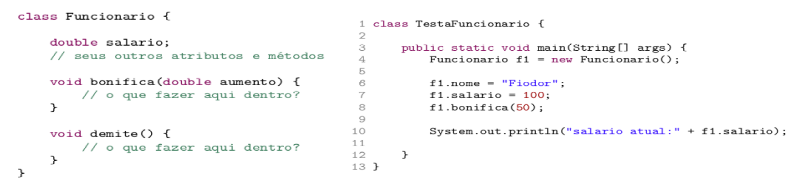
\includegraphics[height=0.3\paperheight]{classes_AEP1.png} \\
% \end{frame}
% \begin{frame}{Atividade - AEP I}
%   \begin{enumerate}
%    \item Transforme o modelo em uma classe Java. Teste-a, usando uma outra 
% classe que tenha o main. Você deve criar a classe do funcionário chamada  
% Funcionario , e a classe de teste você pode nomear como quiser. A de teste deve 
% possuir o método main. Um esboço das classes:
%   \end{enumerate}
%   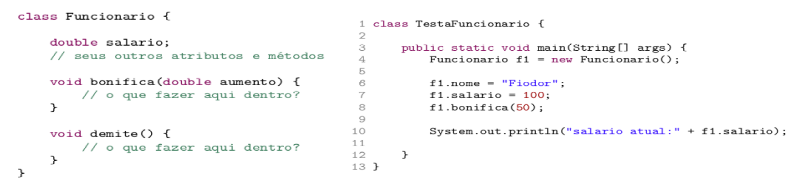
\includegraphics[height=0.3\paperheight]{classes_AEP1.png} \\
% \end{frame}
%-----------------------------------------------------------------------
\section{Leitura recomendada}
 \mode<presentation>{
\begin{frame}{Leitura complementar}
 Para mais informações sobre JAVA, leia:\\
 \begin{columns}
   \begin{column}{0.4\textwidth}
     Java: Como programar\\
     Capítulo 3:\\ 
      \cite{deitel2010java}
   \end{column}
   \begin{column}{0.3\textwidth}
    \begin{center}
  
\includegraphics[height=0.5\paperheight]{fig/aula1/deitel2017java.png} \\
 \end{center}
   \end{column}
 \end{columns}
\end{frame}
}
%----------------------------------------------------------------------------------------------------------------------
 
 \mode<presentation>{\begin{frame}{Referências}%[allowframebreaks]
 \small
 \begin{center}
 	\bibliographystyle{apalike}
	 \bibliography{ref_aula_progI}
 \end{center}
 \end{frame}}


%%%%%%%%%%%%%%%%%% END MATTER %%%%%%%%%%%%%%%%%%
\end{document}